\chapter{Measurements and results}\label{chapter3}
\section{General remarks}
A photoacoustic measurement requires a chopper to modulate the incoming laser at the longitudinal resonance frequency of the chamber, in order to maximize the signal measured by the microphones.

About the microphones, it should be noticed that we didn't know their gain, neither it was possible with our instruments to make a calibration curve. In addition, we thought that understanding in deep the complicated, though interesting, physical processes between the photon absorption and the acoustic wave generation was too far from the general purpose of this work. This implies that, throughout this report, the absorption magnitude signals won't be reported neither with the dimensions of gas absorbance neither with the mechanical dimensions of sound waves. Instead they will be reported in volts, that is, the true (amplified) microphone output that entered the lock-in amplifier. This choice, instead of just using arbitrary units, at least allows us to compare results from different measurements, or even compare our data with those from other groups that used our very same microphones.

\section{Finding chamber resonances}\label{chamber}
The first step of the measurement session was dedicated to find the best resonant frequency. We were told about an approximated length of the internal chamber of 10 cm, hence we expected the first resonating longitudinal mode to be a $\simeq20$ cm long wave. Considering the chamber full of atmospheric pressure \ce{O2} at room temperature, with sound speed 326 m/s this corresponds to a frequency of 1630 Hz.

	\subsection{Open chamber measurement}
We did the measurement stimulating the air inside the chamber through a speaker connected to a waveform generator, and looking at the signal coming from microphones. Since we were not able to insert a speaker inside the chamber (this was small), we excited the open chamber from outside through a hole. The resulting spectrum is shown in \cref{chamberplot}.
\begin{figure}[!t]\centering
% GNUPLOT: LaTeX picture with Postscript
\begingroup
  \makeatletter
  \providecommand\color[2][]{%
    \GenericError{(gnuplot) \space\space\space\@spaces}{%
      Package color not loaded in conjunction with
      terminal option `colourtext'%
    }{See the gnuplot documentation for explanation.%
    }{Either use 'blacktext' in gnuplot or load the package
      color.sty in LaTeX.}%
    \renewcommand\color[2][]{}%
  }%
  \providecommand\includegraphics[2][]{%
    \GenericError{(gnuplot) \space\space\space\@spaces}{%
      Package graphicx or graphics not loaded%
    }{See the gnuplot documentation for explanation.%
    }{The gnuplot epslatex terminal needs graphicx.sty or graphics.sty.}%
    \renewcommand\includegraphics[2][]{}%
  }%
  \providecommand\rotatebox[2]{#2}%
  \@ifundefined{ifGPcolor}{%
    \newif\ifGPcolor
    \GPcolorfalse
  }{}%
  \@ifundefined{ifGPblacktext}{%
    \newif\ifGPblacktext
    \GPblacktexttrue
  }{}%
  % define a \g@addto@macro without @ in the name:
  \let\gplgaddtomacro\g@addto@macro
  % define empty templates for all commands taking text:
  \gdef\gplbacktext{}%
  \gdef\gplfronttext{}%
  \makeatother
  \ifGPblacktext
    % no textcolor at all
    \def\colorrgb#1{}%
    \def\colorgray#1{}%
  \else
    % gray or color?
    \ifGPcolor
      \def\colorrgb#1{\color[rgb]{#1}}%
      \def\colorgray#1{\color[gray]{#1}}%
      \expandafter\def\csname LTw\endcsname{\color{white}}%
      \expandafter\def\csname LTb\endcsname{\color{black}}%
      \expandafter\def\csname LTa\endcsname{\color{black}}%
      \expandafter\def\csname LT0\endcsname{\color[rgb]{1,0,0}}%
      \expandafter\def\csname LT1\endcsname{\color[rgb]{0,1,0}}%
      \expandafter\def\csname LT2\endcsname{\color[rgb]{0,0,1}}%
      \expandafter\def\csname LT3\endcsname{\color[rgb]{1,0,1}}%
      \expandafter\def\csname LT4\endcsname{\color[rgb]{0,1,1}}%
      \expandafter\def\csname LT5\endcsname{\color[rgb]{1,1,0}}%
      \expandafter\def\csname LT6\endcsname{\color[rgb]{0,0,0}}%
      \expandafter\def\csname LT7\endcsname{\color[rgb]{1,0.3,0}}%
      \expandafter\def\csname LT8\endcsname{\color[rgb]{0.5,0.5,0.5}}%
    \else
      % gray
      \def\colorrgb#1{\color{black}}%
      \def\colorgray#1{\color[gray]{#1}}%
      \expandafter\def\csname LTw\endcsname{\color{white}}%
      \expandafter\def\csname LTb\endcsname{\color{black}}%
      \expandafter\def\csname LTa\endcsname{\color{black}}%
      \expandafter\def\csname LT0\endcsname{\color{black}}%
      \expandafter\def\csname LT1\endcsname{\color{black}}%
      \expandafter\def\csname LT2\endcsname{\color{black}}%
      \expandafter\def\csname LT3\endcsname{\color{black}}%
      \expandafter\def\csname LT4\endcsname{\color{black}}%
      \expandafter\def\csname LT5\endcsname{\color{black}}%
      \expandafter\def\csname LT6\endcsname{\color{black}}%
      \expandafter\def\csname LT7\endcsname{\color{black}}%
      \expandafter\def\csname LT8\endcsname{\color{black}}%
    \fi
  \fi
  \setlength{\unitlength}{0.0500bp}%
  \begin{picture}(7200.00,5040.00)%
    \gplgaddtomacro\gplbacktext{%
      \csname LTb\endcsname%
      \put(682,704){\makebox(0,0)[r]{\strut{} 0}}%
      \put(682,1112){\makebox(0,0)[r]{\strut{} 1}}%
      \put(682,1521){\makebox(0,0)[r]{\strut{} 2}}%
      \put(682,1929){\makebox(0,0)[r]{\strut{} 3}}%
      \put(682,2337){\makebox(0,0)[r]{\strut{} 4}}%
      \put(682,2746){\makebox(0,0)[r]{\strut{} 5}}%
      \put(682,3154){\makebox(0,0)[r]{\strut{} 6}}%
      \put(682,3562){\makebox(0,0)[r]{\strut{} 7}}%
      \put(682,3971){\makebox(0,0)[r]{\strut{} 8}}%
      \put(682,4379){\makebox(0,0)[r]{\strut{} 9}}%
      \put(814,484){\makebox(0,0){\strut{} 0}}%
      \put(2012,484){\makebox(0,0){\strut{} 2000}}%
      \put(3210,484){\makebox(0,0){\strut{} 4000}}%
      \put(4407,484){\makebox(0,0){\strut{} 6000}}%
      \put(5605,484){\makebox(0,0){\strut{} 8000}}%
      \put(6803,484){\makebox(0,0){\strut{} 10000}}%
      \put(176,2541){\rotatebox{-270}{\makebox(0,0){\strut{}Magnitude [arbitrary units]}}}%
      \put(3808,154){\makebox(0,0){\strut{}Frequency [Hz]}}%
      \put(3808,4709){\makebox(0,0){\strut{}Open chamber resonances spectrum}}%
      \put(1767,2460){\makebox(0,0){\strut{}1591 Hz}}%
    }%
    \gplgaddtomacro\gplfronttext{%
    }%
    \gplbacktext
    \put(0,0){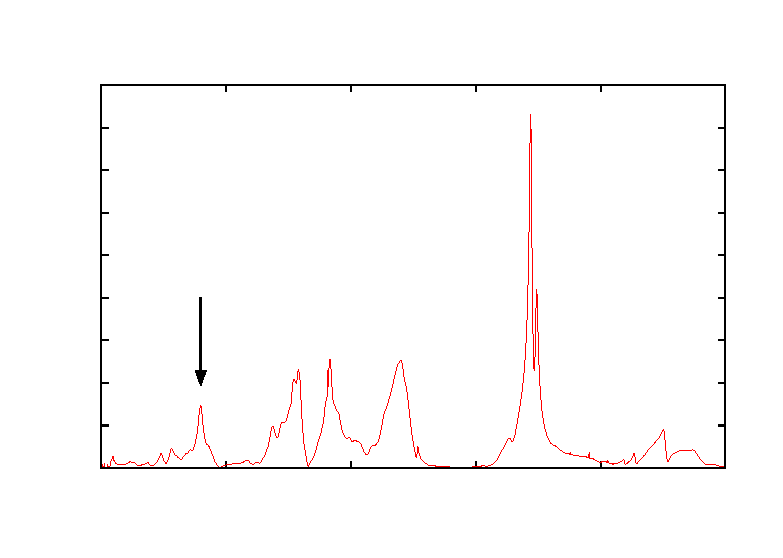
\includegraphics{chamber}}%
    \gplfronttext
  \end{picture}%
\endgroup

\caption{Spectrum of the open chamber, excited with a loudspeaker. The magnitude is set in arbitrary units because this spectrum has been acquired by a software whose unity conversion settings we couldn't control.}
\label{chamberplot}
\end{figure}
In doing this, we differ from the true experimental conditions in three aspects:
\begin{itemize}
\item we have air instead of \ce{O2}
\item we have an open chamber instead of a closed one 
\item the wave signal coming from a small hole aside, instead of being generated in the middle of the chamber.
\end{itemize}

In principle it's easy to correct the spectrum taken in air, in order to apply it to oxygen: in first approximation one has to deal just with a different sound velocity. On the other side, it is more difficult to take into account the acoustic and dynamic modifications the chamber undergoes for being open or closed, as well as for the pressure wave to be originated from a lateral point instead of a diffused volume within the chamber. For these reasons, this cannot be considered as a true spectrum for the chamber we actually used in the absorption measurement. It is nothing more than a useful starting point. Eventually the real resonance frequency had to be experimentally determined with a closed chamber full of oxygen excited from the laser. Also the frequency response of both the loudspeaker and the microphones were unknown, and this could in principle affect the shape of this plot. We looked in a range from 0 to 10 kHz, although we later observed that our chopper wouldn't be able to reach frequencies above few kHz.

We located a clear peak at 1591 Hz, which can attributed to the first longitudinal mode of the chamber, assuming a length $l$ of the chamber slighty greater than the declared 10 cm$$l=\frac{343\mbox{ m/s}}{1591\mbox{ Hz}}\cdot\frac{1}{2}=10.78\mbox{ cm}$$.

		\subsection{Closed chamber measurement}
Starting from the open chamber datum, we injected \ce{O2} in the chamber and started to look for signal by chopping the laser at 1591 Hz. It was promptly clear that there would not be need to further seek for resonances, as the intensity of the signal was high enough even at 1591 Hz, without any correction due to the gas change. We thus decided to delay the search for the acoustic resonance peak in oxygen and proceed with the experiment, in order to save time and give more attention to other issues such as stabilizing the laser emission or look for the oxygen absorption peaks.

Later, at the end of the experiment, we decided that completeness required us to provide the value of maximum resonance with oxygen, even though our measurement were all taken at 1591 Hz. Since the mechanical chopper failed to follow the waveform generator even for the slowest frequency sweep, we couldn't take a spectrum. Changing the frequency by hand we found however the peak at 1512 Hz, where we expected it according to a sound speed in atmospheric pressure oxygen of 323 m/s and a chamber length of 10.78 cm$$f^{\mai{peak}}_{\ce{o2}}=\frac{323\mbox{ m/s}}{2\cdot10.77\mbox{ cm}}\simeq1512\mbox{ Hz.}$$

\section{Looking for the \texorpdfstring{\ce{O2}}{oxygen} peaks}\label{oxygen}
The next step after setting up and optimizing the apparatus was trying to find the best measurement conditions to see the peak. This means to find the frequency of the \ce{O2} absorption peaks, trying the different acoustic resonance frequencies and changing the laser parameters (current, temperature and position of our piezoelectric actuators). 
We were able to measure absorption at various different frequencies, listed in \cref{oxypeaks}:

\begin{table}\centering
\begin{tabular}{|c|}
\hline Wavelength [nm]\\ \hline
686.25 \\ \hline
686.70 \\ \hline
686.75 \\ \hline
686.80 \\ \hline
686.95 \\ \hline
687.05 \\ \hline
687.10 \\ \hline
687.20 \\ \hline
687.25 \\ \hline
687.35 \\ \hline
687.45 \\ \hline
\end{tabular}
\caption{Measured absorption frequencies for \ce{O2} at ambient pressure and temperature.}
\label{oxypeaks}
\end{table}

During this measurements we first noticed the instability of our laser emission in time. For example, when we found some peak at a certain injection current, temperature and piezoelectric position, after some minutes that peak would drift away and we needed to change the piezoelectric position in order to find it again. After a longer time, like a couple of hours, the peak would decrease in intensity and eventually fade completely, forcing us to change temperature or current of the laser
in order to see it again (or to find some other peak). We are going to discuss more accurately this uncontrolled frequency evolution effect in \cref{freedrift}. 

\section{Shape of the peaks}\label{shapeaks}
\label{factorsinfluencingtheshapeofthepeaks}
After having found some absorption peaks and approximately measured their wavelength using the spectrometer, we tried to acquire their shape as well. As seen in \cref{lasersource}, the piezoelectric tunability was too narrow to acquire one whole peak, so it was important to understand which section of the peak we were looking at. This information allowed us to acquire different points of the same absorption peak, by slightly modifying the output frequency of the laser. The frequency instability in time of the laser output was the biggest deal in doing these measurements. 

As explained in \cref{factorshape}, the shape of the peaks was determined by many parameters. This means that we needed to control many of them (at least the three most important) at the same time. To do this we used a computer, together with a data acquisition board exploiting four analog inputs, and we were able to log for every single measurement:
\begin{itemize}
	\item the magnitude of the audio wave coming from the lock-in amplifier
	\item the position of the piezoelectric actuator responsible for the rotation of the grating around the $z$ axis
	\item the wavelength of the highest laser peak, measured by the spectroscope software and converted to an analog signal through the integrated DAC
	\item the intensity of such peak or, depending on the needs, the ratio between the intensity of the peak and its integral (in order to detect multi-modal emission).
\end{itemize}

With this setup, the measurements were performed by sweeping the position of the piezoelectric actuators with the waveform generator. We split them in 3 sessions: single full sweeps, multiple full sweeps and multiple focused sweeps.
\subsection{Factors influencing the shape of the peaks}\label{factorshape}
Before discussing the procedures of measuring the shape of the absorption peaks, it was necessary to analyse which factors had influence on this shape in all the measurements we did. The most important ones were mode hopping, multimodal emission and low-pass deformation, which are discussed in the subsequent paragraphs. Other factors such as
\begin{itemize}
\item variations in the speed of the chopper
\item variations in the oxygen pressure and concentration
\item sample rate of our instruments
\item cable capacitance 
\end{itemize}
should have been not relevant when compared to the first three factors.

\subsubsection{Mode hopping} 
Mode hopping is the factor which most distorted the shape of the measured peaks, limiting us to see only a portion of them. As discussed in \cref{tuna}, the linear range of tunability we can exploit to scan the absorption peak is indeed smaller than the peak width. As the laser exits this interval, a mode jump happens, thus making the photoacoustic resonance to fade away. We got around this by logging the wavelength of the emission peak, measured with the spectrometer and calculated by the \textit{Avaspec}\textsuperscript{\copyright} software in real time\footnote{within a response time less than 10$^{-1}$ s.}. Superimposing this data to the acoustic magnitude ones we could distinguish between the parts of the peaks which really corresponded to the absorption peak shape and the parts affected by mode-hopping.

\subsubsection{Multimodes}
The ECDL didn't always emit light on a single wavelength, but often it would emit in 2 or 3, rarely on 4, different wavelengths at the same time. One or more of these emissions could correspond to one of the oxygen absorption lines, thus generating a measurable photoacoustic effect (\cref{multimodes}). This situation rose the problem that the relative intensity of the various emitted wavelengths was not constant even within the tunability range. Therefore the shape of the peak in such situation could be distorted by the change of intensity. In addition, our apparatus could log and register only the wavelength and intensity of the strongest emitted peak, even when the laser was not emitting in a single mode. This made very difficult to distinguish between single-mode and multi-mode emissions just looking at the recorded data. 
Indeed the only way we had to suppose a multi-modal emission according to the recorded data was looking for
\begin{itemize}
\item fast jumps between two wavelengths competing in being the main one
\item decreases in the main peak intensity or in the intensity-peak integral ratio, though difficult because these two parameters were quite noisy.
\end{itemize}
The best solution we found, however, was to personally attend to the measurements and observe the etalon interference pattern to detect multi-modal emissions. Also it was important to try many different sets of laser parameters, in order to avoid multimodal emissions which contained absorption wavelengths.

\begin{figure}
\includegraphics[width=\linewidth, draft=\foto]{eps/multimode.eps}
\caption{We can see two different absorption peaks, both of them appearing during a multimodal laser emission. The first peak corresponds to a wavelength of 687.40 nm but suddenly jumps to a wavelength of 686.65 nm, while the second corresponds to an absorption wavelength of 687.30 nm but jumps back and forth several times between to the frequency of 687.05 nm. This means that the laser is emitting in at least two different modes at the same time and while initially one of the two is the strongest, after a bit the other becomes higher and the spectrometer starts indicating it as the main peak. In such a situation the shape of the peak is severely deformed by the changes in intensity of the various modes.
Laser parameters: 29.10\cel; 73.23 mA.}
\label{multimodes}
\end{figure} 

\subsubsection{Noise and lock-in low pass filter}
The lock-in amplifier we used contained an adjustable low pass filter to control the output signals. A higher time constant allows to filter out more noise, but on the other side it would correspond to a lower slew rate of the signal. This deformed the shape of the peaks, especially when the signal changed abruptly during a mode hop or in fast sweep measurement. After several attempts we found that a time constant of 1 second gave a quite stable output without requiring us to make too slow measurements.
\subsection{Single full sweeps} 
In this kind of measurement, we set the laser diode temperature and injection current, waited about 15 minutes to get emission stability, and started sweeping the piezoelectric crystal along its full driving range (0-150 V), using a linear ramp function with a period of about 11 minutes. This kind of experiment showed all the different absorption peaks available with that choice of laser parameters, and also to study the periodicity of the laser modes with respect to the grating position.

\medskip
\cref{primopicco,moltipicchi} show the result of this first session of measurements. In \cref{fullsweep1} a full sweep of the piezoelectric actuators made the laser to hop its emission mode many times. But only few of those modes met the absorption peak of the oxygen, thus resulting in a high signal. In \cref{fullsweep2} the same modes gives a much lower signal: we moved far away from the absorption peak maximum, even though we didn't change any of the parameters. This is due to the laser frequency drift discussed in \cref{freedrift}.

In \cref{moltipicchi} we slightly changed one of the laser parameters: the diode temperature. The whole modes pattern is now completely reshuffled with respect to \cref{primopicco}, and the full sweep of the piezoelectric actuators shown in \cref{bevified} now highlights three different absorption peaks. A closer observation, in \cref{magnified}, permits to fully appreciate this, as well as to see the signal deformation due to the factors discussed in \cref{factorshape}.
\begin{figure}[!hptb]\centering
\subfigure[Absorption, maximum of a peak. Laser parameters: 29.16 $^\circ$C; 73.23 mA.\label{fullsweep1}]{\includegraphics[width=\linewidth, height=9.5cm, draft=\foto]{eps/660s_first.eps}} 
\subfigure[Absorption, tail of a peak. Laser parameters: 29.16 $^\circ$C; 73.23 mA.\label{fullsweep2}]{\includegraphics[width=\linewidth, height=9.5cm, draft=\foto]{eps/660s_second.eps}}
\caption{Photoacoustic absorption of a $\simeq$ 687.0 nm peak. The wavelength shift between the two plots is of the order of $10^{-2}$ nm, thus it's not visible on the scale. The noisy parts at $\simeq220$ s are due to the fast backwards ramp of the sweeping.}\label{primopicco}
\end{figure}

\begin{figure}[!hptb]\centering
\subfigure[Laser parameters: 29.06 $^\circ$C; 73.23 mA.\label{bevified}]{\includegraphics[width=\linewidth, height=9.5cm, draft=\foto]{eps/660s_third_normal.eps}} 
\subfigure[Magnification of the previous plot.\label{magnified}]{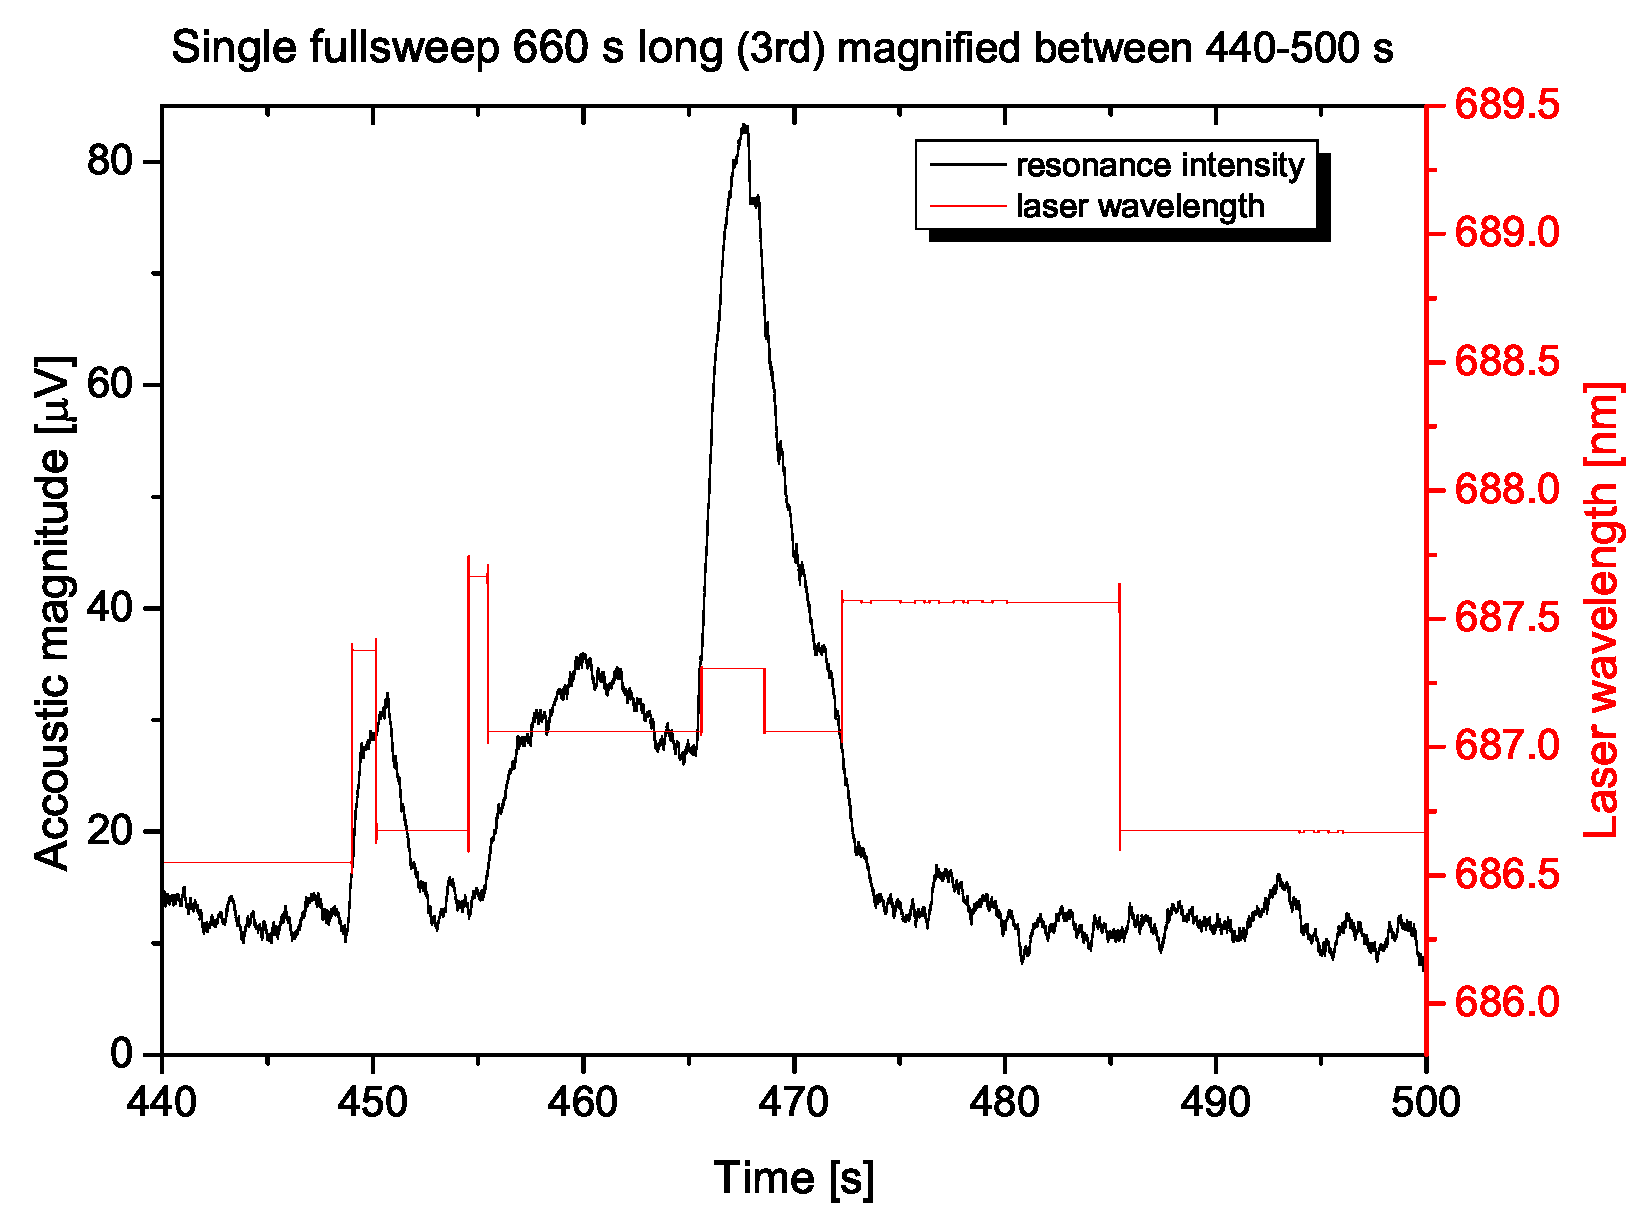
\includegraphics[width=\linewidth, height=9.5cm, draft=\foto]{eps/660s_third_magni.eps}}
\caption{In this measurement, the laser diode temperature is 0.1 $^\circ$C lower than \cref{primopicco}. We notice 3 different absorption wavelengths: 687.30, 687.35, 687.05 nm. Here are visible the deformations we studied in\cref{factorshape}}\label{moltipicchi}
\end{figure} 

\medskip
Looking at the peak wavelength plots we noticed that the laser mode jumping is somehow periodical with respect to the piezoelectric sweeping voltage. That is, for portions of the sweep about 50-100 V large the modes hop from one to another according to a constant pattern.
This can be easily seen in \cref{hoppattern}, which shows both the wavelength of the main emission peak and its intensity, during part of the sweep shown in \cref{fullsweep1}. The pattern, followed clearly for at least a couple of periods, is shown in \cref{tabrutta}.

\begin{figure}[!hbpt]\centering
\includegraphics[width=\linewidth, height=10cm, draft=\foto]{eps/periodicityofhops.eps}
\caption{We can see that the laser follows the same hopping pattern for several seconds, corresponding to a piezoelectric voltage sweep of 75 V.}
\label{hoppattern}
\end{figure}

\begin{table}[!hbpt]\centering
	\begin{tabular}{|c|c|}
	\hline	Time interval [s]&Wavelength [nm]\\
		\hline
0&687.45\\ \hline%339
5&686.60\\ \hline
21&687.40\\ \hline
24&687.65\\ \hline
27&687.05\\ \hline
39&687.30\\ \hline
39&687.05\\ \hline
41&687.55\\ \hline
55&686.95\\ \hline
	\end{tabular}
\caption{Example of hopping pattern. The time intervals are calculated from the beginning of \cref{hoppattern}, 339 s.}
\label{tabrutta}
\end{table}

%DA QUI A QUI STAVA QUI
% (scrivere di come in effetti sto aumento virtuale non sia quasi mai stato possibile da misurare a causa deella deformaz dei picchi dovuti alle instabilità o al semplice fatto che la nuova parte visibile è irrilevante (non contiene picco). 

	\subsection{Multiple full sweeps}
Since these measurement took quite a long time every sweep, doing repeated measurements most of time resulted in unmatchable data, because of the uncontrolled evolution we already mentioned. The influence of such uncontrolled factors exhibited however a random behaviour, so that, after some trials, we were able to get a unique \textquotedblleft lucky\textquotedblright measurement of 3 subsequent sweeps which matched almost perfectly. This is shown in \cref{3sweep}.

All the other attempts, instead, resulted in severe changes of the resonance pattern between one sweep and another. Studying the pattern of the wavelength vs voltage graphic helps in realizing that this difference is not to be ascribed to the photoacoustic part of the experiment (oxygen concentration/pressure, laser alignment) but is rather due to a change in the laser emission wavelength pattern. \cref{3missweep,7sweeps} provide meaningful examples of this behaviour.
The change in the wavelength pattern is better shown in \cref{focus}, where we will focus
on shorter multiple sweeps around a single absorption peak.
\begin{landscape}
\begin{figure}[!bhtp]\centering
\includegraphics[height=\textheight, draft=\foto]{eps/3sweepsmatching.eps}
\caption{Three subsequent 0-150 V sweeps, of duration of 11 minutes each. Red: acoustic signal magnitude vs time and actuators voltage. Green: time projection. Blue: voltage projection. Notice that in the voltage projection the matching between the peaks of different sweeps in almost perfect. Laser parameters: 29,50 $^\circ$C; 80,01 mA.}
\label{3sweep}
\end{figure}\vfill
\end{landscape}

\begin{landscape}
\begin{figure}[!bhtp]\centering
\includegraphics[height=\textheight, draft=\foto]{eps/3mismatching.eps}
\caption{Despite these measurements are taken faster then usual (5 minutes each 0-150 V sweep) there is a big mismatch between the three sweeps. This mismatch is more evident in the magnitude vs voltage projection, where the peaks seem to be double-peaks. The time projections shows instead that they are
single peaks. Laser parameters: 27,68\cel; 80,01 mA}
\label{3missweep}
\end{figure}\vfill
\end{landscape}

\begin{landscape}
\begin{figure}[!bhtp]\centering
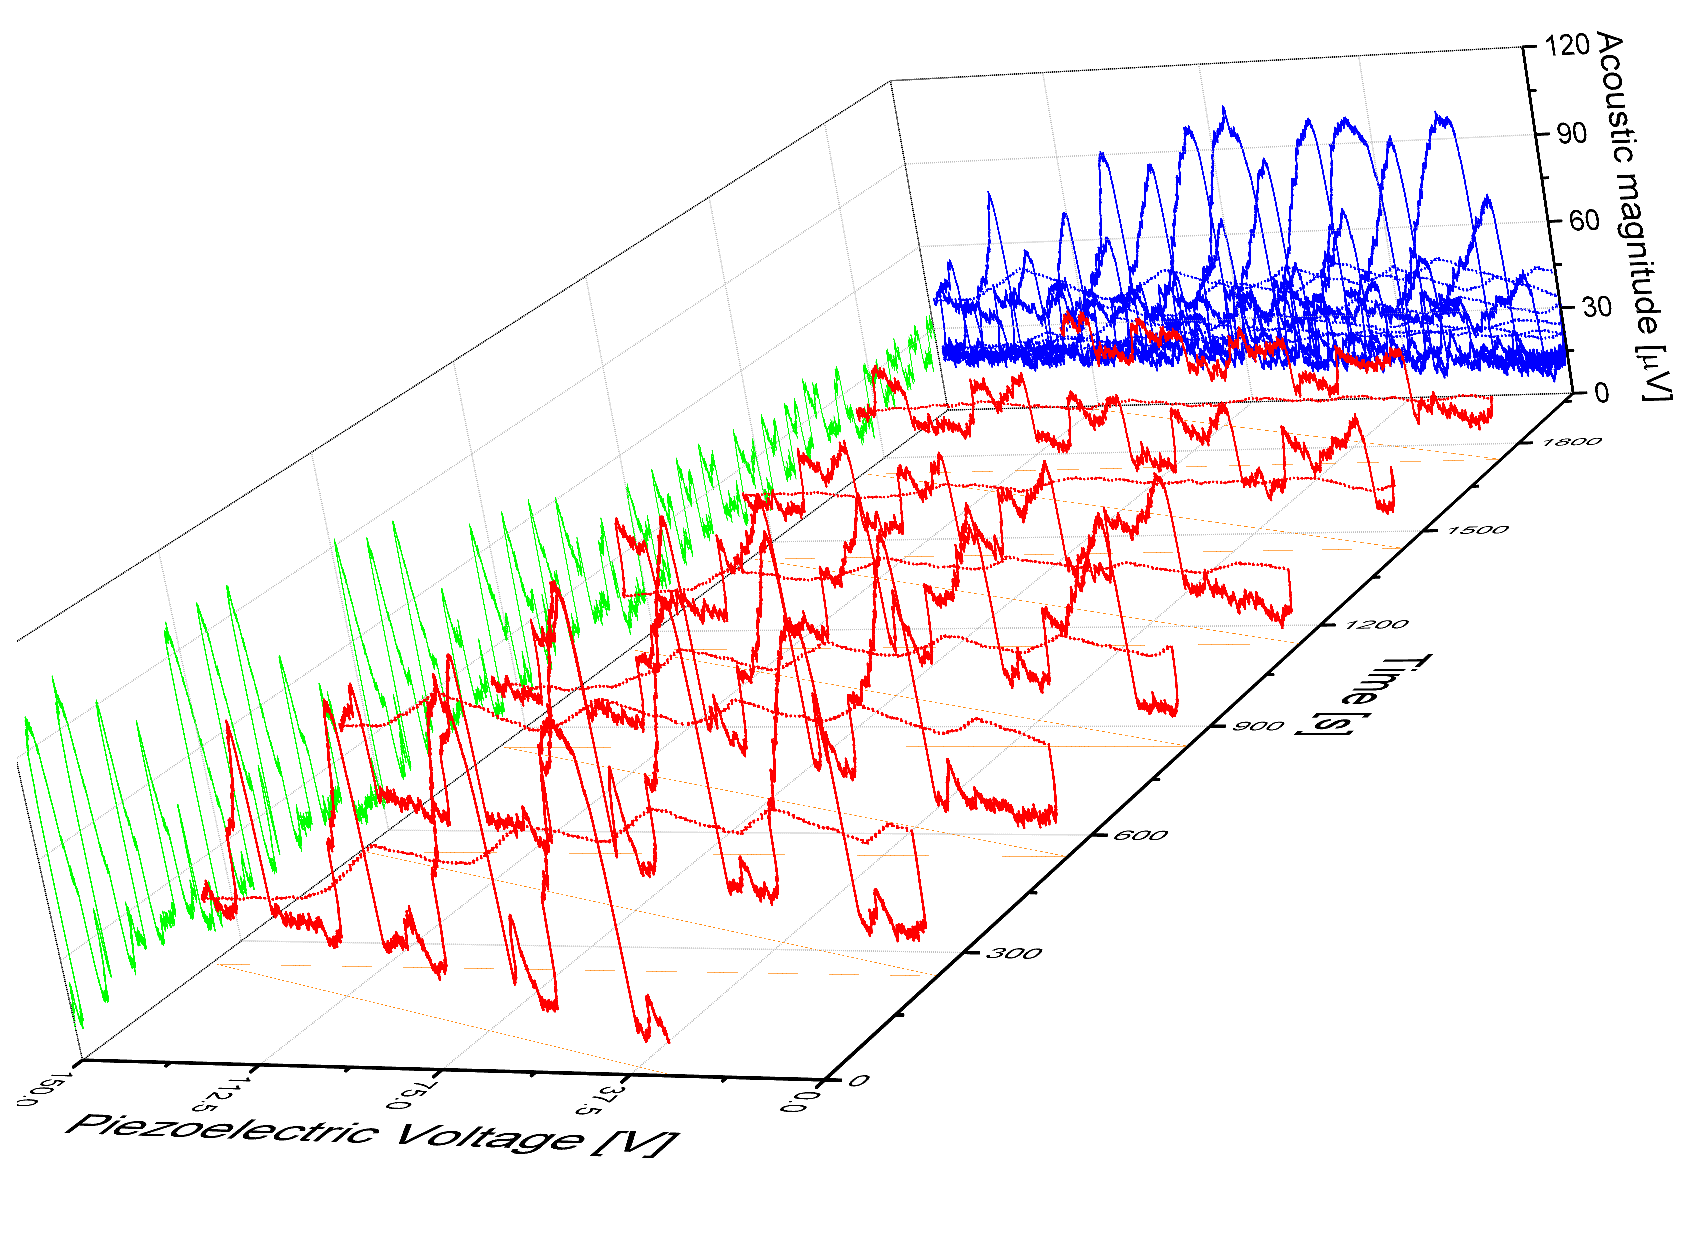
\includegraphics[height=\textheight, draft=\foto]{eps/7sweeps.eps}
\caption{In this measurement it is shown not only the fact that the peaks shift in voltage with time but can completely fade away after some minutes. Laser parameters: 25,03\cel; 80,01 mA}
\label{7sweeps}
\end{figure}\vfill
\end{landscape}
  
	\subsection{Multiple focused sweeps}\label{focus}
Another measurement methodology we used exploited repeated single-peak sweeps instead of 
full 0 to 150 V sweeps. This was intended to better study both the absorption peak shape and the evolution caused by external factors. In this kind of measurements it is also possible to use uncontrolled evolution at our advantage, since sometimes it allowed to increase the tunability range before a mode hopping. \cref{multisweep} shows how repeating a measurement of the same peak changed the part of the peak we were able to see. In \cref{multisweep1} the part of the peak we were able to see decreased after each sweep, while in \cref{multisweep2} the scanned part of the peak instead increased \textquotedblleft thanks\textquotedblright to the uncontrolled time evolution.
In both of these examples we see that we could not usually measure the "tunability range" using the spectrometer data, but still we are able to see that the voltage to laser mode dependence changes with time. 

\begin{figure}[!phtb]\centering
\subfigure[Laser parameters: 27,68\cel; 80,01 mA\label{multisweep1}]{\includegraphics[width=\linewidth, height=9.5cm, draft=\foto]{eps/multisweeps1.eps}}
\subfigure[Laser parameters: 25.03\cel; 80,01 mA\label{multisweep2}]{\includegraphics[width=\linewidth, height=9.5cm, draft=\foto]{eps/multisweeps2.eps}}
\caption{The resonance frequency shifts after every measurement, changing the part of the peak (in black) we were able to scan and decreasing the maximum measurable intensity.}
\label{multisweep}
\end{figure}

In order to better study how the voltage to wavelength output changed with time we plotted all the sweeps of \cref{multisweep1} on a voltage/intensity graphic, thus getting \cref{nonshiftedpeaks}, and subsequently shifted them by the voltage required to match the part of the peak which most likely corrisponded to the oxygen absorption peak (see \cref{factorsinfluencingtheshapeofthepeaks}), getting \cref{shiftedpeaks} as result.

\begin{figure}
\subfigure[Same measurement as \cref{multisweep1}, but rearranging the data to split the 10 different sweeps.\label{nonshiftedpeaks}]{\includegraphics[width=\linewidth, height=9.5cm, draft=\foto]{eps/multiunmatched.eps}}
\subfigure[Each measurement is now shifted of the values listed below in \cref{peakshifts} in order to match the part of the peak corresponding to the oxygen absorption peak.\label{shiftedpeaks}]{\includegraphics[width=\linewidth, height=9.5cm, draft=\foto]{eps/multimatched.eps}}
\caption{In order to compare the different signal peaks, and relate them to the same absorption peak, we shifted them manually during the data processing.}
\label{grafishifti}
\end{figure}

In order to make the edges of the peak match, we had to shift the various peaks of the values listed in \cref{peakshifts}
\begin{table}[!htbp]\centering
\begin{tabular}{|c|c|c|}
\hline
N of peak & Shift [V] & $\Delta$Shift [V] \\ \hline
2 & -0.04 & -0.04 \\ \hline
3 & -0.065 & -0.025 \\ \hline
4 & -0.1 & -0.035 \\ \hline
5 & -0.12 & -0.02 \\ \hline
6 & -0.142 & -0.022 \\ \hline
7 & -0.157 & -0.015 \\ \hline
8 & -0.185 & -0.028 \\ \hline
9 & -0.195 & -0.01 \\ \hline
10 & -0.22 & -0.025 \\ \hline
\end{tabular}
\caption{Shifts of peaks in \cref{shiftedpeaks} with respect to the first peak and to the precedent peak.}
\label{peakshifts}
\end{table}

Looking at these data we could notice that, while the evolution is monotonic during our whole measurement, its speed is not constant, i.e. every peak has to be shifted a different amount with respect to the previous one.

\begin{figure}[!tphb]\centering
\includegraphics[width=\linewidth, draft=\foto]{eps/multimatchedwavelength.eps}
\caption{In this graphic the wavelength corresponding to each sweep has already been shifted of the same amount as the data in graph \cref{shiftedpeaks}.}
\label{multiwave}
\end{figure}

From the wavelength to voltage graph we can also see that, even after having shifted the sweeps in order to match the peak edges, the mode hopping from 687.35 nm (not corresponding to any absorption peak) to 687.41 nm is not happening at the same voltage in the various sweeps. This means that the environmental factors evolution cannot be modelled with a simple voltage drift (otherwise the voltage could find correction by just a voltage shift), but suffers the influence of more complicated factors.
More efforts to study this kind of evolution have been described in \cref{freedrift}.

\section{Free laser drift analysis}\label{freedrift}
\subsection{Free evolution}
To study how the evolution worked we acquired some measurements of the laser output using the spectrometer and the etalon, while keeping constant all the laser parameters (current, temperature and piezoelectric voltage). At first we took a short term measurement lasting 20 minutes. But we understood that the evolution was quite slow, and that this first measurement was too short to be meaningful. We then took a second long term measurement, lasting a night time, in order to see whether a stable regime was reached. These are shown in \cref{senzaniente}.

The first thing we noticed was that the mode hopping due to the uncontrolled evolution followed the same pattern as the mode hopping due to the piezoelectric movement (see an example in \cref{hoppattern,tabrutta}). This suggested us the idea that one of the factors which generating this evolution could be a movement of the grating of the ECDL, allegedly caused by thermal expansion of the cage system holding it. 

\begin{figure}[!hptb]\centering
\subfigure[Twenty minutes measurement. No equilibrium configuration is reached, nor clear pattern is visible. Laser parameters: 29,50 $^\circ$C; 80,00 mA.\label{senzaniente20}]{\includegraphics[width=\linewidth, height=9.5cm, draft=\foto]{eps/20minuteshops.eps}} 
\subfigure[Twelve hours measurement. A low frequency pattern appears, and this looks very similar to the mode hopping pattern due to the grating movements. Laser parameters: 25,03 $^\circ$C; 80,01 mA.\label{senzaniente12h}]{\includegraphics[width=\linewidth, height=9.5cm, draft=\foto]{eps/nighttime.eps}}
\caption{Laser free drift measurements.}
\label{senzaniente}
\end{figure} 
 
\subsection{Heating- and cooling-induced evolution}

In order to confirm the fact that the evolution depends mainly on temperature (of the cage system or of the air) effects we put a tungsten lamp near the ECDL and turned it on. As we can see from \cref{lampdrift}, turning on the lamp increased the speed of the evolution a lot. After keeping the lamp on for a while we turned it off and took another measurement. This time we observed an evolution pattern almost as fast as the one with the lamp on, but with a reverse pattern. We interpreted this a signal that the system is cooling down.

\begin{figure}[!t]\centering
\includegraphics[width=\linewidth, draft=\foto]{eps/lampandnot.eps}
\caption{During the measurements with the lamp turned on we were  eventually able to see the difference in the minimum and maximum wavelength of the same mode after some drifts, as represented in the next graphic. Laser parameters: 27,68\cel; 80,01  mA.}
\label{lampdrift}
\end{figure}

\begin{figure}[!b]\centering
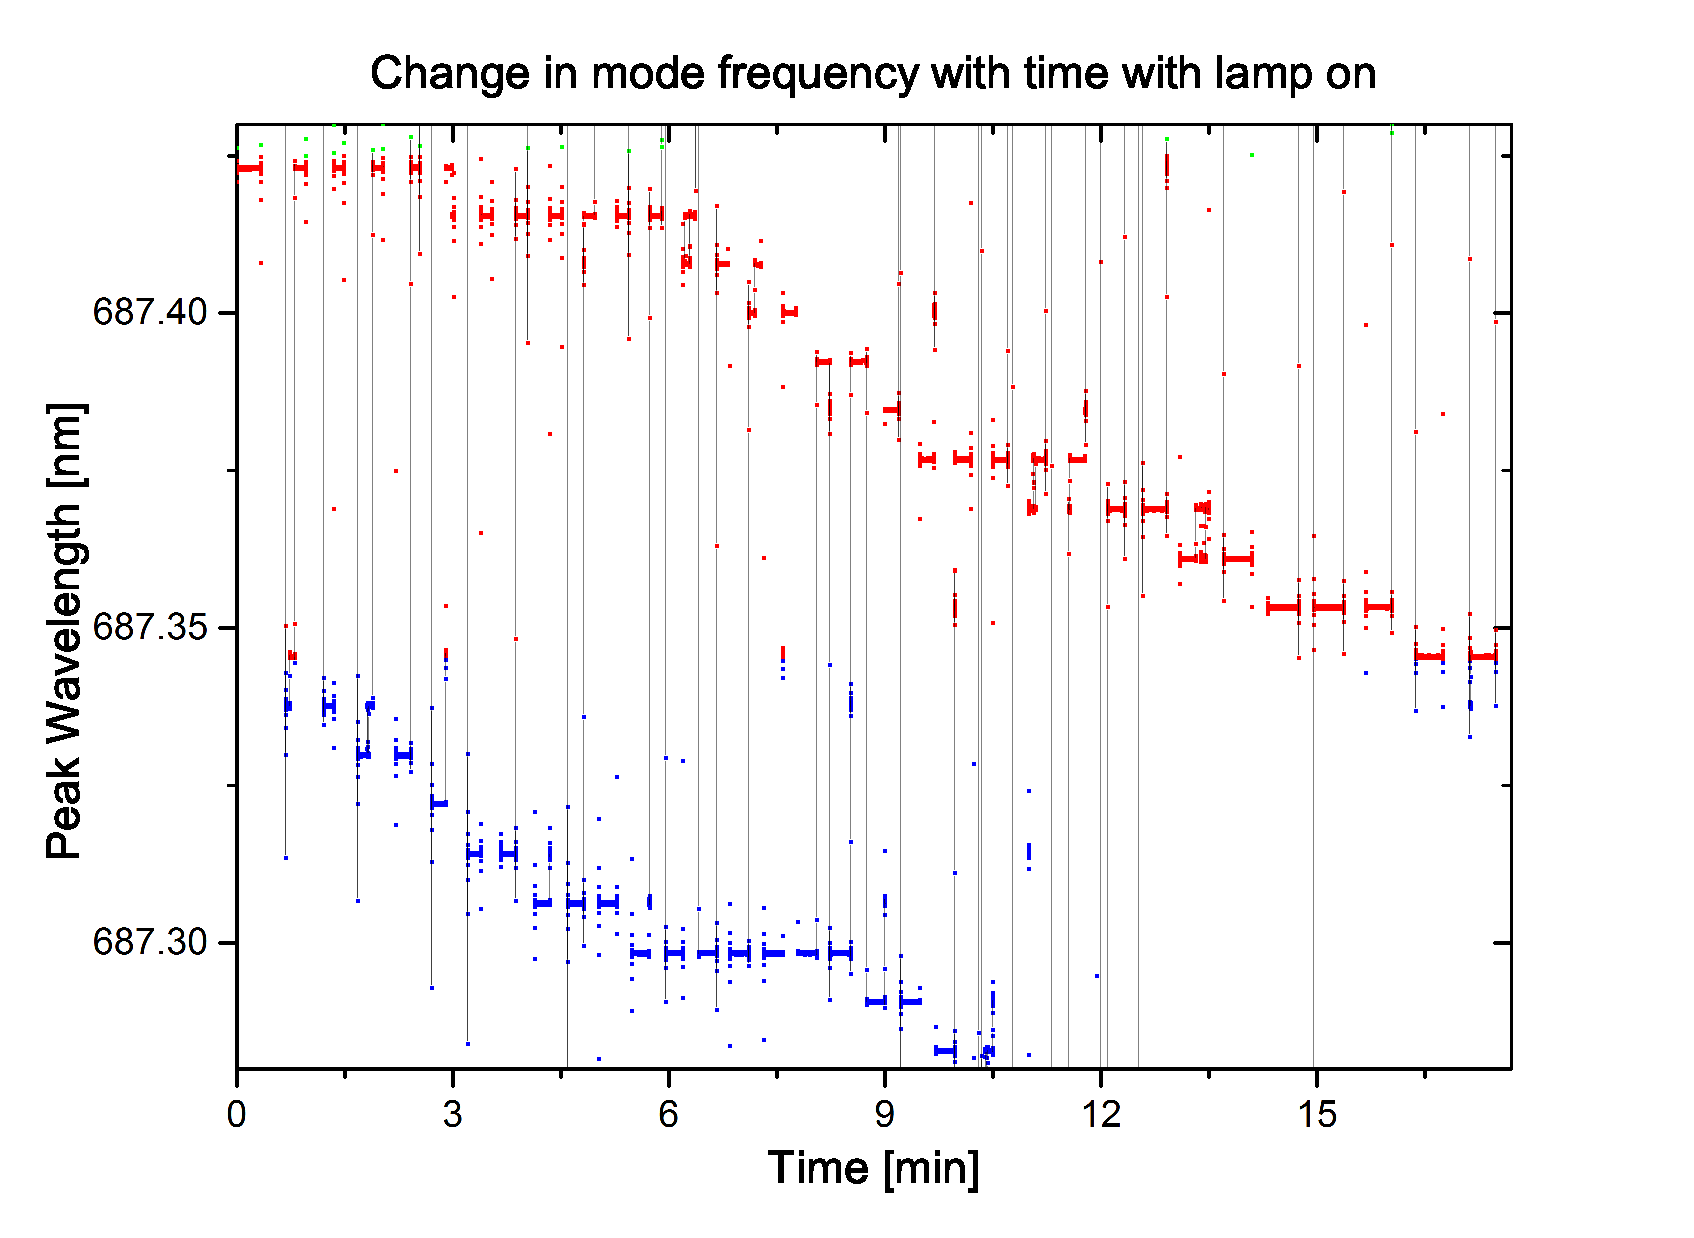
\includegraphics[width=\linewidth, draft=\foto]{eps/modedrift.eps}
\caption{The wavelength of both of the mode shown here decreases after some periods of hopping. Laser parameters: 25.03\cel; 80.01 mA.}
\label{modedrift}
\end{figure}
 
\subsection{Tunability change measurement}
Since the resolution of our spectrometer was usually not good enough to distinguish a tunability change in time, we used the etalon to take a measurement similar to the tunability measurement of a mode (687.45 nm) several times, measuring the minimum  and maximum wavelength before a mode hop for about two hours.
The results in \cref{minmaxshift} show how not only the minimum and maximum piezoelectric voltages, but also the position of the etalon interference pattern change in time. Considering that the etalon FSR is of the order of 3-4 microseconds (on the video camera PAL signal), we found that the min-max drift is of the order of about one half as the tunability found in \cref{tuna}.
%is of the order of the Ghz/timeunitnoncostante
%l'incertità dei dati dovuta alla larghezza dei picchi (che conta un tot) nella tabella è dei soliti 40ns/2radq2log2 cioè di circsa 2.12330450072005E-007 s ma forse un po' menosispera. l'errore di risoluz dell'oscillocoso sarebbe invece 40 ns /radq12).
\begin{table}[!p]
\begin{tabular}{|c|c|c|c|c|c|}
\hline
Time [min] & $\Delta$Min [ns] & Min volt. [V] & $\Delta$Max [ns] & Max volt. [V] & Tunab. [ns] \\ \hline
%0 & 9.677 & 3 & 9.678 & 17 & 560 \\ \hline
15 & 0 & 19 & 180 & 24 & 720 \\ \hline
30 & 250 & 20 & $<$40 & 27 & 500 \\ \hline
50 & 260 & 23 & 260 & 29 & 480 \\ \hline
95 & -330 & 23 & -360 & 29 & 440 \\ \hline
135 & 330 & 29 & 220 & 38 & 560 \\ \hline
\end{tabular}
\caption{Shifts of the maximum and minimum positions on the oscilloscope of the 687.45 nm mode. As discussed in \cref{tuna}, the uncertainty on the time measurement is estimated to be $\simeq$ 40 ns.}
\label{minmaxshift}
\end{table}
